\chapter{Differential Equations}
In physics we encounter differential equations all the time. In fact the whole programme of classical mechanics is to develop a second order differential equation using Newton's laws of motion and then solving it.\\Sometimes these are ordinary
differential equations in one variable (abbreviated ODEs). More often the equations are
partial differential equations (PDEs) in two or more variables. Simply we can say , differential equations is a relation between a function and its derivatives.
\begin{definition}
	A differential equation is an equation which involves independent and dependent variables and their derivatives or differentials.
\end{definition}
\begin{example}
	\hspace{1cm}
\begin{itemize}
		\item $\frac{dy}{dx}={4x-2}$
		\item $\frac{d^{2}y}{dx^{2}}=5\frac{dy}{dx}+10$
		\item $(1+\frac{dy}{dx})^{3}=k\frac{dy}{dx}$
		\item $\frac{dy}{dx}+xy=x^{3}y^{3}$
		\item $\frac{\partial^{2}y}{\partial^{2} x}=\frac{1}{c^{2}} \frac{\partial^{2}y}{\partial^{2} x} $
		\item $\frac{\partial u}{\partial t}=\frac{\partial u}{\partial x}+\frac{\partial u}{\partial y}$
	\end{itemize}
\end{example}
\section{{Types of differential equation}}
There are mainly two types of differential equations,
	\begin{itemize}
	\item \textbf{Ordinary differential equations.}\par A differentnial equation involving derivatives with respect to a single variable is called an ordinary differential equation. 
	\\\\
	\textbf{General form:} $\frac{d y}{d x}=f(x, y)=-\frac{P(x, y)}{Q(x, y)}$
	\begin{example}
		\begin{align*}
		F&=m\frac{d v}{dt}\\
		\frac{dy}{dx}+x&= 1
		\end{align*}
	\end{example}
	\item \textbf{Partial differential equations.}\par A differential equation involving partial derivatives with respect to more than one independent variable is called a partial differential equation.
	\begin{example}
		\begin{align*}
		\intertext{\textbf{Poisson's equation:}}
		\nabla^{2}\psi&= \frac{\rho}{\epsilon_{0}}\\
		\left( \frac{\partial ^{2}}{\partial x^{2}}+\frac{\partial ^{2}}{\partial y^{2}}+\frac{\partial ^{2}}{\partial z^{2}}\right)\psi &= \frac{\rho}{\epsilon_{0}}\qquad (\text{In cartesian coordinate system.})
		\intertext{\textbf{Schrodinger Equation:}}
		\left(-\frac{h^{2}}{2 m} \nabla^{2}+V\right) \psi&=i \hbar \frac{\partial \psi}{\partial t}
		\end{align*} 
	\end{example}
	\end{itemize}
\section{Order and Degree of a differential equation}
\textbf{Order:}\\The order of a differential equation is the highest differential in the equation.\\\\
\textbf{Degree:}\\The degree of a differential equation is the power of the highest differential in the equation.
\begin{example}
	\hspace{0.5cm}
	\begin{itemize}
		\item $\left(\frac{\partial^{2} y}{\partial x^{2}}\right)^{2}+\left(\frac{\partial y}{\partial x}\right)-\left(\frac{\partial^{3} y}{\partial x^{3}}\right)=x y$\hspace{0.5cm}Order=2 ,Degree=2
		\item   $ L \frac{d^{2} q}{d t^{2}}+R \frac{d q}{d t}+\frac{q}{c}=E \sin \omega t$\hspace{1cm}Order=2 ,Degree=1
		\item $\frac{dy}{dx}+xy=x^{3}y^{3}$ \hspace{2.7cm}Order=1 ,Degree=1
		\item $\left(\frac{\mathrm{d}^{2} \mathrm{y}}{\mathrm{d} \mathrm{x}^{2}}\right)^{3}=\left[1+\left(\frac{\mathrm{dy}}{\mathrm{dx}}\right)^{4}\right]^{5}$
	 \hspace{1.1cm} Order=2 ,Degree =3
	 \item $\frac{d^{3} y}{d x^{3}}-\left(\frac{d y}{d x}\right)^{\frac{1}{2}}=0$ \hspace{2.3cm} Order=3 ,Degree=2
	\end{itemize}
\end{example}
\begin{exercise}
Find the order and degree of the given differential equations, 

\begin{enumerate}
	\item $\frac{d^{3} y}{d x^{3}}-\left(\frac{d y}{d x}\right)^{\frac{1}{2}}=0$
	\item $\left[1+\frac{d^{2} y}{d x^{2}}\right]^{\frac{3}{2}}=a \frac{d^{2} y}{d x^{2}}$
\end{enumerate}
\end{exercise}
\begin{answer}\hspace{0.5cm}
\begin{enumerate}
	\item Here we need to eliminate the radical sign.
	For this write the equation as
	\\\begin{align*}
	\frac{d^{3} y}{d x^{3}}&=\left(\frac{d y}{d x}\right)^{\frac{1}{2}}\\\text{ Squaring both sides, we get  }\\\left(\frac{d^{3} y}{d x^{3}}\right)^{2}&=\frac{d y}{d x}\\
	\therefore \quad  \text{Order} =3,\text{degree} =2
	\end{align*}
	\item Here we eliminate the radical sign. For this write the equation as
	
   \begin{align*}
	\left[1+\frac{d^{2} y}{d x^{2}}\right]^{\frac{3}{2}}&=a \frac{d^{2} y}{d x^{2}}
	\\\text{ Squaring both sides, we get  }\\\left[1+\frac{d^{2} y}{d x^{2}}\right]^{3}&=a^{2}\left(\frac{d^{2} y}{d x^{2}}\right)^{2}\\
	\therefore \quad  \text{Order} =2,\text{degree} =3
	\end{align*}
\end{enumerate}
\end{answer}
\begin{note}
The direction of a curve at a particular point is given by the tangent line at that point and the slope of the tangent is given by $\frac{dy}{dx}$ at that point.	
\end{note}
\section{First order differential equation}
An equation of the general form
$$
\frac{d y}{d x}=-\frac{f(x, y)}{g(x, y)}
$$
Is said to be a first order differential equation.The equation contains first and no higher derivatives. The only derivative here $\frac{d y}{d x}$ is a total or ordinarry derivative not a partial one.
\section{Geometrical meaning of First order First degree differential equations}
\begin{wrapfigure}{r}{0.5\textwidth}
	\begin{center}
		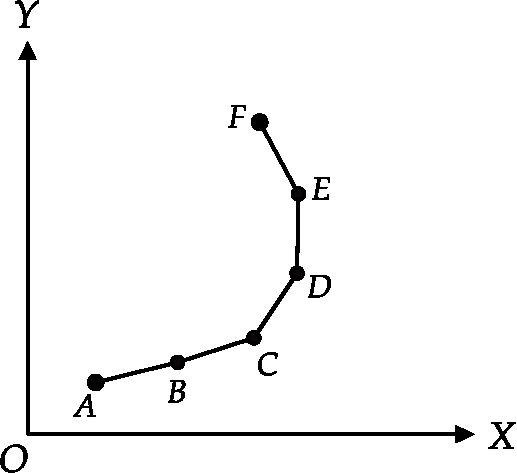
\includegraphics[width=0.25\textwidth]{03-crop}
	\end{center}
	\caption{Geometrical meaning of Differential equation}
\end{wrapfigure}
The solution of every  first order first degree differential equations represent a family of curves.
\\\\Let, $f\left(x, y, \frac{d y}{d x}\right)=0$\quad  represents a differential equation of  first order and first degree.\\\\
Taking $A\left(x_{0}, y_{0}\right)$ as an initial point,we
can find $\frac{d y}{d x}$ at $A\left(x_{0}, y_{0}\right)$. And with the help of that we can draw the tangent at the point $A$.\\\\
On the tangent line take a neighbouring point $B\left(x_{1}, y_{1}\right)$. Find $\frac{d y}{d x}$ at the point $B\left(x_{1}, y_{1}\right)$and draw the tangent at $B$. And in this way draw another tangent at the point $C$ on the tangent line $B$ . Similarly draw, some more tangents by taking the neighbouring points on them. Again we take another starting point $A^{\prime}\left(x_{0}^{\prime}, y_{0}^{\prime}\right)$. We can draw another curve starting from
$A^{\prime} .$ In this way we can draw a number of curves. They form a smooth curve. \\
That is the given difrential equation represents a family of curves.

\section{Solution of a differential equation}
A solution of a differential equation is any relation
between variables which is free of derivatives and which
satisfies the differential equation.\\\\
\textbf{General solution:}\\ A general solution is the solution in which the number
of arbitrary constants and the order of the differential
equation are same.\\\\
\textbf{Particular solution:}\\ A particular solution is the solution which can be
obtained by giving particular values to arbitrary constants of general solution.

\section{Solution of First order differential equations}
The solutions of first order differential equations are obtained by various methods,
\section{ Method of seperation of variables}
If all functions of $x$ and $d x$ can be arranged on one side and $y$ and $d y$ on the other side, then the variables are separable. The solution of this equation is found by integrating the functions of $x$ and $y$.
$$f(x) d x=g(y) d y\Longrightarrow
\int f(x) d x=\int g(y) d y+C
$$
\textbf{\large Method of solving:}
\begin{enumerate}
	\item  Separate the variables as $f(x) d x=g(y) dy$.
    \item Integrate both sides as $\int f(x) d x=\int g(y) d y$.
    \item  Add an arbitrary constant $C$ on R.H.S.
\end{enumerate}
\begin{exercise}
Solve	$\cos (x+y) d y=d x$
\end{exercise}
\begin{answer}[H]
	\begin{align*}
		\cos (x+y) d y&=d x \\
		\frac{d y}{d x}&=\sec (x+y)\\
		\text{  Let, }x+y&=z\\
		\text{  Then, }1+\frac{d y}{d x}=\frac{d z}{d x} \quad & \Rightarrow \quad \frac{d y}{d x}=\frac{d z}{d x}-1 \\
		\frac{d z}{d x}-1=\sec z \quad &\Rightarrow \quad  \frac{d z}{d x}=1+\sec z\\
		\text{Separating the variables, we get, }\\\frac{d z}{1+\sec z}&=d x\\
		\text{On integrating,}\\
		\int \frac{\cos z}{\cos z+1} d z&=\int d x\\
		\int\left[1-\frac{1}{\cos z+1}\right] d z&=x+C \\
		\int\left[ 1-\frac{1}{2 \cos ^{2} \frac{z}{2}-1+1}\right]  d z&=x+C \\
		\int\left(1-\frac{1}{2} \sec ^{2} \frac{z}{2}\right) d z&=x+C\\
		\int\left(1-\frac{1}{2} \sec ^{2} \frac{z}{2}\right) d z&=x+C\\
		z-\tan \frac{z}{2}&=x+C  \\
		x+y-\tan \frac{x+y}{2}&=x+C\\
		 y-\tan \frac{x+y}{2}&=C 
	\end{align*}
\end{answer}
\begin{exercise}
	Solve $e^{d y / d x}=(x+1) ;$ given $y=3$ at $x=0$
\end{exercise}
\begin{answer}
	Taking log of both sides we get, 
	\begin{align*}
		\frac{d y}{d x}=\ln (x+1)\quad &\Rightarrow \quad d y=\ln (x+1) d x\\\text{on integration }, \\\int d y=\int 1 \cdot \ln (x+1) d x \quad &\Rightarrow \quad y=x \ln (x+1)-\int \frac{x}{(x+1)} d x+C\\
		y&=x \ln (x+1)-\int \frac{(x+1)-1}{(x+1)} d x+C\\ y&=x \ln (x+1)-\int \frac{(x+1)}{(x+1)} d x+\int \frac{1}{(x+1)} d x+C\\&=x \ln (x+1)-x+\ln (x+1)+C\\y&=(x+1) \ln (x+1)-x+C\\\text{Given: at,}\ x&=0 \quad y=3 \Rightarrow \quad C=3\\
		\text{Therefore,}\ y&=(x+1) \ln (x+1)-x+3
	\end{align*}
	
\end{answer}
\section{Solution of Homogeneous differential equation}
Homogeneous equations are of the form,
$$
\frac{d y}{d x}=\frac{f(x, y)}{g(x, y)}
$$
Where $f(x, y)$ and $g(x, y)$ are homogeneous functions of the same degree in $x$ and $y$. Homogeneous functions are those in which all the terms are of $n^{th}$  degree.\\\\ 
\textbf{\large Method of solving}
\begin{enumerate}
	\item  Put, $y=v x,$ then $\frac{d y}{d x}=v+x \frac{d y}{d x}$.
	\item  Separate $v$ and $x$ and then integrate.\\\\
	$
	\begin{aligned}
	 \frac{d y}{d x}&=f(y / x) \\
	\Rightarrow  \hspace{1.1cm}y / x&=v \\
	\Rightarrow \hspace{0.3cm}\frac{d v}{f(v)-v}&=\frac{d x}{x} \\
	\Rightarrow  \int \frac{d v}{f(v)-v}&=\log x+C 
	\end{aligned}
	$
\end{enumerate}
\begin{exercise}
	Solve the differential equation $\left(x^{2}-y^{2}\right) d x+2 x y$ $d y=0,$ given that $y=1$ when $x=1$
\end{exercise}
\begin{answer}

	\begin{alignat*}{2}
		\left(x^{2}-y^{2}\right) d x+2 x y d y&=0\\
			\left(x^{2}-y^{2}\right) d x&=-2 x y d y \\
			\frac{d y}{d x}=-\frac{x^{2}-y^{2}}{2 x y}&=\frac{y^{2}-x^{2}}{2 x y}\\
			\text{Putting  } y=v x  \quad &\text{and} \quad \frac{d y}{d x}=v+x \frac{d v}{d x}\\
			\text{ We get}
			\quad v+x \frac{d v}{d x}&=\frac{v^{2} x^{2}-x^{2}}{2 x \cdot v x}\\
			\Rightarrow \hspace{2cm}\quad v+x \frac{d v}{d x}&=\frac{v^{2}-1}{2 v}\\
			\Rightarrow\hspace{2.7cm} x \cdot \frac{d v}{d x}&=\frac{v^{2}-1}{2 v}-v\\&=\frac{v^{2}-1-2 v^{2}}{2 v}\\&=-\left[\frac{v^{2}+1}{2 v}\right]\\
			\Rightarrow \hspace{1.5cm}\quad \frac{2 v}{v^{2}+1} \cdot d v&=-\frac{d x}{x}, \quad x \neq 0\\
			\Rightarrow \hspace{1.1cm}\quad \int \frac{2 v}{v^{2}+1} \cdot d v&=-\int \frac{d x}{x}\\
			\Rightarrow \hspace{1.3cm}\quad \log \left(v^{2}+1\right)&=-\log |x|+c\\
			\Rightarrow \quad \log \left(v^{2}+1\right)+\log |x|&=\log c\\
			\Rightarrow \hspace{1.5cm}\quad\left(v^{2}+1\right)|x|&=c\\
			\text{Now, putting }v&=y / x\\
			\left(y^{2} / x^{2}+1\right)|x|&=c \\
			\Rightarrow \left(x^{2}+y^{2}\right)&=c|x|\\\text{	Which is similar to } x=1 \quad \text{and} \quad y=1, \text{we get,}c&=2\\\text{Putting value of} \quad c&=2 ,\text{We get}\\x^{2}+y^{2}&=2 x \text { or } x^{2}+y^{2}=2(-x)\\x=1 &\quad \text{and}\quad y=1 \\\text{Do not satisfy}\quad x^{2}+y^{2}&=2(-x) \\\text{Hence,}\quad x^{2}+y^{2}&=2 x \quad \text{is the required solution.}
	\end{alignat*}
\end{answer}

\subsection{Equations reducible to homogeneuos form}
Let a differential equation be,
$$
\frac{d y}{d x}=\frac{a x+b y+c}{A x+B y+C}
$$
\textbf{Type-1}\\

\begin{align*}
\text{If, in the above equation,}\quad\frac{a}{A}&\neq\frac{b}{B}\\\text{Then we can substitute}\quad x=X+h\quad&,\quad y=Y+k,\text{($h, k$ being constants)}\\
\text{The given differential equation reduces to}\\
\frac{d Y}{d X}&=\frac{a(X+h)+b(Y+k)+c}{A(X+h)+B(Y+k)+C}\\&=\frac{a X+b Y+a h+b k+c}{A X+B Y+A h+B k+C}\\
\text{Choose $h, k$ so that} \quad a h+b k+c&=0\\
A h+K k+C&=0\\
\text{Then the given equation becomes homogeneous}\\\frac{d Y}{d X}&=\frac{a X+b Y}{A X+B Y}
\end{align*}
\textbf{Type-2}\\
\begin{align*}
\text{If}\ \frac{a}{A}&=\frac{b}{B},\\
\text{Then the value of $h, k$ will not be finite.}\\
\frac{a}{A}&=\frac{b}{B}=\frac{1}{m}\\
A=a m\quad, \quad B&=b \mathrm{~m}\\
\text{The given equation becomes}\quad\frac{d y}{d x}&=\frac{a x+b y+c}{m(a x+b y)+C}
\end{align*}
 Now put $a x+b y=z$ and apply the method of variables separable.
 \begin{exercise}
 	Solve $(x+2 y)(d x-d y)=d x+d y$
 \end{exercise}
\begin{answer}
	\begin{align*}
	(x+2 y)(d x-d y)&=d x+d y \\\Rightarrow(x+2 y-1) d x-(x+2 y+1) d y&=0\\
	\Rightarrow  \frac{d y}{d x}&=\frac{x+2 y-1}{x+2 y+1}\\
	\text { Let } x+2 y&=z \\ 1+2 \frac{d y}{d x}&=\frac{d z}{d x} \\ \frac{d z}{d x}&=\frac{3 z-1}{z+1}\quad  (\text{Since, $ \frac{d y}{d x}=\frac{x+2 y-1}{x+2 y+1}$})\\
	\int \frac{z+1}{3 z-1} dz &=\int dx\\
	\text{L.H.L}&=\int \frac{z+1}{3 z-1} dz\\
	\intertext{multiply numerator and denominator by 3, we get, }
		\text{L.H.L}&=\int \frac{1}{3} \frac{(3z+3)}{(3 z-1)} dz\\
		&=\int \frac{1}{3} \frac{(3z-1+4)}{(3 z-1)} dz\\
		&=\int \frac{1}{3} \frac{(3z-1)+4}{(3 z-1)} dz\\
		&=\int \frac{1}{3}\left\lbrace  \frac{(3z-1)}{(3 z-1)}+ \frac{4}{(3 z-1)}\right\rbrace dz\\
		&=\int \left\lbrace  \frac{1}{3}+  \frac{1}{3} \frac{4}{(3 z-1)}\right\rbrace dz\\
		&=\int \left\lbrace  \frac{1}{3}+  \frac{4}{9} \frac{1}{(3 z-1)}\right\rbrace dz\\
		&=\frac{1}{3} z+\frac{4}{9} \ln (3 z-1)+c
		\intertext{Then,}
		\int \frac{z+1}{3 z-1} dz &=\int dx \Rightarrow	\quad 
		\frac{1}{3} (x+2y)+\frac{4}{9} \ln (3 x+6 y-1)=2x+c\\
		3 x-3 y+a&=2 \ln (3 x+6 y-1)\\
		4 \ln (3 x+6 y-1)&=(6 x-6y)+c\\
	2 \ln (3 x+6 y-1)&=(3 x-3y)+c\\
\end{align*}
\end{answer}
\section{Linear equation of first order}
If a differential equation has its dependent variables and its derivatives occur in the first degree and are not multiplied together, then the equation is said to be linear. The standard equation of a linear equation of first order is given as
$$
\frac{d y}{d x}+P y=Q
$$
Where $P$ and $Q$ are functions of $x$.

\begin{align*}
\text { Integrating factor }&=(\text { I.F. })=e^{\int P \cdot d x} \\
\Rightarrow y \cdot e^{\int P \cdot d x}&=\int Q \cdot e^{\int P \cdot d x} d x+C \\
\Rightarrow \hspace{0.3cm}y(\mathrm{I.F.})&=\int Q(\mathrm{I.F.}) d x+C\\
\end{align*}

\begin{exercise}
	Solve the differential equation $\frac{d y}{d x}-\frac{y}{x}=2 x^{2}, x>0$.
\end{exercise}
\begin{answer}
	we know,
	
	\begin{align*}
		\frac{d y}{d x}+\left(\frac{-1}{x}\right) y &=2 x^{2}\\
		\frac{d y}{d x}+P y=Q, \text { where } P &=-\frac{1}{x} \text { and } Q=2 x^{2}\\
		I.F&=e^{\int P \cdot d x}=e^{\int-1 / x \cdot d x}\\&=e^{-\log x}=e^{\log x^{-1}}=x^{-1}=\frac{1}{x}\\
		\text{Multiplying both sides with $I.F$, we get}\\\frac{1}{x} \cdot \frac{d y}{d x}-\frac{1}{x^{2}} \cdot y&=2 x\\
		\text{Integrating both sides w.r.t. $x,$ we get}\\y \cdot\left(\frac{1}{x}\right)&=\int 2 x \cdot d x+C \\
		\Rightarrow \quad y \cdot \frac{1}{x}&=x^{2}+C\\\Rightarrow\hspace{0.9cm} y&=x^{3}+C x, x>0 \quad \text{is the required solution.}
	\end{align*}
\end{answer}
\subsection{Equations reducible to linear form}
The differential equation of the form,
$$\frac{dy}{dx}+p(x)y=f(x)y^{n}$$is called the Bernoulli's equation or equation reducible to linear form.
It can be done by dividing by $y^{n}$ and substituting $\frac{1}{y^{n-1}}=z$
\begin{alignat*}{2}
&\frac{1}{y^{n}} \frac{d y}{d x}+\frac{1}{y^{n-1}} P&&=Q\\&\text{Put}\quad \frac{1}{y^{n-1}}&&=z\\&\frac{(1-n)}{y^{n}} \frac{d y}{d x}&&=\frac{d z}{d x} \\ &\Rightarrow \quad \frac{1}{y^{n}} \frac{d y}{d x}&&=\frac{d z}{1-n}\\
&\frac{1}{1-n} \frac{d z}{d x}+P z&&=Q \quad \text{or}\\& \frac{d z}{d x}+P(1-n) z&&=Q(1-n)
\end{alignat*}
Which is a linear equation and can be solved easily.
\begin{exercise}
	Solve $\frac{d y}{d x}+x y=x^{3} y^{3}$
\end{exercise}
\begin{answer}We have,
	\begin{align*}
\frac{d y}{d x}+x y&=x^{3} y^{3}\\
\frac{1}{y^{3}} \frac{d y}{d x}+\frac{x}{y^{2}}&=x^{3}\\
	\text{putting}\quad \frac{1}{y^{2}}&=z \\\Rightarrow \quad \frac{-2}{y^{3}} \frac{d y}{d x}&=\frac{d z}{d x} \quad \Rightarrow \quad \frac{1}{y^{3}} \frac{d y}{d x}=\frac{-1}{2} \frac{d z}{d x}\\\therefore \quad-\frac{1}{2} \frac{d z}{d x}+x z&=x^{3} \qquad\Rightarrow \quad \frac{d z}{d x}-2 x z=-2 x^{3}\\
	\mathrm{\therefore I.F.}=e^{-\int 2 x d x}&=e^{-x^{2}}\\
	z e^{-x^{2}}&=-2 \int x^{3} e^{-x^{2}} d x\\
	\text{Let}\quad  -x^{2}&=t \Rightarrow-2 x d x=d t\\
	z e^{-x^{2}}&=\int t e^{t} d t=t e^{t}-e^{t}+c\\
	\text{put}\quad z=y^{-2} \text{and}\quad t=-x^{2}\\
	\therefore \frac{e^{-x^{2}}}{y^{2}}&=-x^{2} e^{-x^{2}}-e^{-x^{2}}+c\\
	\frac{1}{y^{2}}&=-x^{2}-1+C e^{x^{2}}
	\end{align*}
\end{answer}
\section{Exact differential equations}
A differential equation of the form , $Mdx+Ndy=0$ is said to be  exact if it satisfy the following condition,$$\frac{\partial \boldsymbol{M}}{\partial \boldsymbol{y}}=\frac{\partial N}{\partial \boldsymbol{x}}$$
$\frac{\partial M}{\partial \boldsymbol{y}}\quad-\quad$Differential co-efficient of $M$ with respect to $y$ keeping $x$ constant\\
$\frac{\partial N}{\partial \boldsymbol{x}}\quad-\quad$Differential co-efficient of $N$ with respect to $x$, keeping $y$ constant.\\\\
\textbf{\large Method of solving:}\\
\textbf{Step 1:} Integrate $M$ w.r.t. $x$ keeping $y$ constant\\
\textbf{Step 2:} Integrate w.r.t. $y$, only those terms of $N$ which do not contain $x$.\\ \textbf{Step 3:} Result of 1 + Result of 2 = Constant.
\begin{exercise}
	Solve $\left(x^{2}+2 x y\right) d x+\left(x^{2}+y^{2}\right) d y=0$
\end{exercise}
\begin{answer}
	\begin{align*}
	\text{Here,}\quad M=\left(x^{2}+2 x y\right) \quad &\text{and}\quad N=\left(x^{2}+y^{2}\right)\\\Rightarrow \frac{\partial M}{\partial y}&=2 x\\\text{and}\quad
	\frac{\partial N}{\partial x}&=2 x\\
	\text{Hence, the given equation is exact}\\
	\int\left(x^{2}+2 x y\right) d x+\int y^{2} d y&=c\\\frac{x^{3}}{3}+x^{2} y+\frac{y^{3}}{3}&=C\\\text { The solution is: } \\\int\left(x^{2}+2 x y\right) d x+\int y^{2} d y=c=\frac{x^{3}}{43}+x^{2} y+\frac{y^{3}}{3}&=6\end{align*}
\end{answer}
\subsection{Equations reducible to Exact form}
A differential equation which is not exact can be reduced to exact form  by multiplying it by a constant , here the integrating factor.\\
\textbf{Type 1:} If $ \frac{\frac{\partial M}{\partial y}-\frac{\partial N}{\partial x}}{N}\text { is a function of } x \text { alone, say } f(x), \text { then } \mathrm{I.F}=e^{\int f(x) d x}$\\
\textbf{Type 2:} If $\frac{\frac{\partial N}{\partial x}-\frac{\partial M}{\partial y}}{M}$ is a function of $y$ alone, say $f(y),$ then
$
\mathrm{I.F} =e^{\int f(y) d y}
$
\begin{exercise}
	Solve $(2 x \log x-x y) d y+2 y d x=0$
\end{exercise}
\begin{answer}
\begin{align*}
M &=2 y,\quad N=2 x \log x-x y\notag\\
\frac{\partial M}{\partial y}&=2,\quad\frac{\partial N}{\partial x}=2(1+\log x)-y\\
\text { Here, }\notag \\
\quad \frac{\frac{\partial M}{\partial y}-\frac{\partial N}{\partial x}}{N}&=\frac{2-2-2 \log x+y}{2 x \log x-x y}\\&=\frac{-(2 \log x-y)}{x(2 \log x-y)}=-\frac{1}{x}=f(x)\notag\\\text { I.F. }&=e^{\int f(x) d x}=e^{\int-\frac{1}{x} d x}\\&=e^{-\log x}=e^{\log x^{-1}}=x^{-1}=\frac{1}{x}\\
&\text{On multiplying the given differential equation by}  \frac{1}{x}, \text{we get}\\
\frac{2 y}{x} d x+(2 \log x-y) d y&=0 \\ \Rightarrow \quad \int \frac{2 y}{x} d x+\int-y d y&=c \\
\Rightarrow  \qquad\quad 2 y \log x-\frac{1}{2} y^{2}&=c
\end{align*}
\end{answer}
\section{Orthogonal trajectories and Family of curves}
Given a one-parameter family of plane curves, it's orthogonal trajectories are another
one-parameter family of curves, each one of which is perpendicular to all the curves in the
original family. For instance, if the original family consisted of all circles having center at the origin, it's orthogonal trajectories would be all rays (half-lines) starting at the origin.
\begin{definition}
	Two families of curves are such that every curve of either family cuts each curve of the other family at right angles. They are called orthogonal trajectories of each other.
\end{definition}
Orthogonal trajectories arise in different contexts in applications. If the
original family represents the lines of force in a gravitational or electrostatic field, its orthogonal trajectories represent the equipotentials, the curves along which the gravitational or electrostatic potential is constant.
\begin{example}\hspace{1cm}
	\begin{enumerate}
		\item The path of an electric field is perpendicular to equipotential curves.
		\item  In fluid flow, the stream lines and equipotential lines are orthogonal trajectories.
		\item The lines of heat flow is perpendicular to isothermal curves.
	\end{enumerate}
\end{example}
\subsection{Finding orthogonal trajectories to the curve}
Let a family of curves be given by the equation
$$
g(x, y)=C
$$
Where $C$ is a constant. For the given family of curves, we can draw the orthogonal trajectories, that is another family of curves $f(x, y)=C$ that cross the given curves at right angles.
\subsubsection{Method of solving}
\textbf{Family of curves given ,then to find orthogonal trajectories.}
\begin{enumerate}
	\item  By differentiating the equation of curves find the differential equations in the form $f\left(x, y, \frac{d y}{d x}\right)=0$
	\item  Replace $\frac{d y}{d x}$ by $-\frac{d x}{d y}$\\ ($ m_{1}m_{2}=-1$, where,$m_{1}$=given family,$m_{2}$=orthogonal  family)
	\item  Solve the differential equation of the orthogonal trajectories i.e., $f\left(x, y,-\frac{d x}{d y}\right)=0$
\end{enumerate}
\textbf{Orthogonal trajectories given , then to find Family of curves .}
\begin{enumerate}
	\item Solve the differential equation of the orthogonal trajectory $f\left(x, y,\frac{d x}{d y}\right)=0$ using appropriate method.
\end{enumerate}
\begin{note}
	\textbf{Self-orthogonal:}. If the family of orthogonal trajectory is the same as the given family of curves,then it's called self orthogonal.
\end{note}
\begin{exercise}
	 Find the orthogonal trajectories of the family of straight lines  $y=C x,$  where  $C$  is a parameter.
\end{exercise}
\begin{answer}
	\begin{align*}
	\text{we have,}\quad y&=C x\\
	\text{differentiating the given equation we get}\\
	dy&=cdx\\
	dy&=\frac{y}{x}dx\quad(\because c=\frac{y}{x})\\
	\frac{dy}{dx}=\frac{y}{x}\\
	{\frac{dy}{dx}}_{(ortho)}&=\frac{-x}{y}\\
	\text{ using variable separable method}\\
	(-xdx&=ydy)\\
	\int-xdx&=\int ydy\\
	-\frac{x^{2}}{2}&=\frac{y^{2}}{2}+C\\
		\frac{x^{2}}{2}+\frac{y^{2}}{2}&=C\\
		x^{2}+y^{2}&=2C\Longrightarrow \text{Represents the family of circles}
	\end{align*}
\end{answer}
\begin{exercise}
	Find the family of curves of the given trajectory,	$\frac{dy}{dx}=\frac{x}{y}$
\end{exercise}
\begin{answer}
\begin{align*}
\text{given},\frac{dy}{dx}&=\frac{x}{y}\\
\text{using variable seperable method, we get}\\
\int xdx&=\int ydy\\
\frac{x^{2}}{2}&=\frac{y^{2}}{2}+C\\
\frac{x^{2}}{2}-\frac{y^{2}}{2}&=C\\
x^{2}-y^{2}&=2C\Longrightarrow \text{family of hyperbolas}
\end{align*}
\end{answer}
\section{Second order differential equations}
\subsection{Linear differential equation}
If the degree of the dependent variable and all derivatives is one, such differential equations are called linear differential equations.
\begin{example}\hspace{0.5cm}
	\begin{enumerate}
		\item $2\frac{d^{2} y}{d x^{2}}+3\frac{d y}{d x}+4 y=x^{2}+x+1$
		\item $ \frac{d^{2} x}{d x^{2}}-\frac{d y}{d x}-3 y=x$
		\item $2 \frac{d^{2} x}{d t^{2}}-\frac{d x}{d t}-3 x=f(t)$
	\end{enumerate}
\end{example}
\subsection{Non-Linear differential equation}
If the degree of the dependent variable and / or its derivatives are of greater than 1 such differential equations are called non-linear differential equations.
\begin{example}\hspace{0.5cm}
	\begin{enumerate}
		\item $\frac{d^{2} y}{d x^{2}}+\frac{d y}{d x}+y^{2}=\sin x$
		\item  $\frac{d^{2} y}{d x^{2}}+2\left(\frac{d y}{d x}\right)^{2}+y^{2}=e^{x}$
		\item  $\left(\frac{d^{2} x}{d t^{2}}\right)^{2}+\frac{d x}{d t}+x=f(t)$
	\end{enumerate}
\end{example}
\subsection{Homogeneous differential equation}
A differential equation of the form
$y^{\prime \prime}+P(x) y^{\prime}+Q(x) y=F(x)$, is said to be  homogeneous if $F(x)= 0$
\begin{example}
	\hspace{0.5cm}
	\begin{enumerate}
		\item 	$\frac{d^{2} y}{d x^{2}}-6 \frac{d y}{d x}+13 y=0$
		\item $\frac{d^{2} y}{d x^{2}}+2\left(\frac{d y}{d x}\right)^{2}+y^{2}=0$
	\end{enumerate}

\end{example}
\subsection{Nonhomogeneous differential eqaution} A differential equation of the form
$y^{\prime \prime}+P(x) y^{\prime}+Q(x) y=F(x)$, is said to be  non-homogeneous if $F(x)\neq 0$
\begin{example}
\hspace{0.5cm}
\begin{enumerate}
	\item 	$\frac{d^{2} y}{d x^{2}}-6 \frac{d y}{d x}+ y=x^{2}+2$
	\item $\frac{d^{2} y}{d x^{2}}+2\left(\frac{d y}{d x}\right)^{2}+y^{2}=e^{x}$
\end{enumerate}
\end{example}
\section{Linear independance and dependance of solutions}
Two solutions of a differential equation, $ y_{1}(x)$ and $ y_{2}(x)$ are said to be linearly independant if \\$$Ay_{1}(x)+By_{2}(x)\neq 0 $$ given, $ A\neq0 \quad\text{and}\quad B\neq0$
\subsection{Wronskian}
A first-order homogeneous ODE has only one linearly independent solution. This is meant in the following sense. "If two solutions are linearly dependent, by definition they satisfy $a y_{1}(x)+b y_{2}(x)=0$ with nonzero constants $a, b$ for all values of $x$". If the only solution of this linear relation is $a=0=b$, then our solutions $y_{1}$ and $y_{2}$ are said to be linearly independent.
\\To prove this theorem, suppose $y_{1}, y_{2}$ both solve the homogeneous ODE. Then,
\begin{equation*}
\frac{y_{1}^{\prime}}{y_{1}}=-p(x)=\frac{y_{2}^{\prime}}{y_{2}} \quad \Rightarrow \quad W(x) \equiv y_{1}^{\prime} y_{2}-y_{1} y_{2}^{\prime} \equiv 0
\end{equation*}
The functional determinant $W$ is called the \textbf{Wronskian of the pair $y_{1}$, $y_{2}$}. We now show that $W \equiv 0$ is the condition for them to be linearly dependent. Assuming linear dependence, that is.
\begin{equation*}
a y_{1}(x)+b y_{2}(x)=0
\end{equation*}
In matrix form, the Wronskian of two functions $y_{1}(x)$ and $y_{2}(x)$ is given by,
\begin{equation}
W\left(y_{1}, y_{2}, x\right)=\left|\begin{array}{ll}
y_{1}(x) & y_{2}(x) \\
y_{1}^{\prime}(x) & y_{2}^{\prime}(x)
\end{array}\right|=y_{1}(x) y_{2}^{\prime}(x)-y_{1}^{\prime}(x) y_{2}(x)
\end{equation}
\begin{enumerate}
	\item If $W\left(y_{1}, y_{2}, x\right)=0,$ then $y_{1}(x)$ and $y_{2}(x)$ are linearly dependent.
	\item If $W\left(y_{1}, y_{2}, x\right) \neq 0,$ then $y_{1}(x), y_{2}(x)$ are linearly independent.
\end{enumerate}
\begin{note}
	The wronskian of a differential equation can also be written as,
	$$ W(t)=e^{-\int p(x)dx}$$
	\end{note}
\begin{exercise}
Consider two solutions $\mathrm{x}_{1}(\mathrm{t})$ and $\mathrm{x}_{2}(\mathrm{t})$ of the differential equation $\frac{d^{2} x(t)}{d t^{2}}+x(t)=0, t>0$, such that $x_{1}(0)=1,\left.\frac{d x_{1}(t)}{d t}\right|_{t=0}=0, x_{2}(0)=0,\left.\frac{d x_{2}(t)}{d t}\right|_{t=0}=1$. The Wronskian $W(t)=\left|\begin{array}{ll}x_{1}(t) & x_{2}(t) \\ \frac{d x_{1}(t)}{d t} & \frac{d x_{2}(t)}{d t}\end{array}\right|$ at $t=\frac{\pi}{2}$ is,	
\end{exercise}
\begin{answer}
	The wronskian of a differential equation can also be written as,
	\begin{align*}
	W(t)&=e^{-\int p(x)dx}\\
	\text{But here,}\quad  p(x)&=0\\
	\text{Then,} \quad W(t)&=e^{0 \ dx}=1\\
	\text{So,}\quad W(\frac{\pi}{2})&=1
	\end{align*}
\end{answer}
\section{Linear Second Order Differential Equations With Constant Coefficients}
The general form of the linear differential equation of second order is
$$
\frac{d^{2} y}{d x^{2}}+P \frac{d y}{d x}+Q y=R
$$
Where $P$ and $Q$ are constants and $R$ is a function of $x$ or constant.\begin{note}\textbf{Differential operator:}\\
	A differential operator can be represented as,\quad $D=\frac{d}{dx}$
\\Then a differential equation can be written  in terms of differntial operators as,
\begin{align*}
D^{2} y+P D y+Q y&=R \\ \left(D^{2}+P D+Q\right) y&=R\\
\text{Where,}\quad D y&=\frac{d y}{d x}, \ \text{and}\ D^{2} y=\frac{d^{2} y}{d x^{2}}
\end{align*}

$\frac{1}{D}$ stands for the operation of integration.	
\end{note}
\section{Solution of Second order homogeneous differential equation.}

\subsection{Method of solving}
\begin{enumerate}
	\item Let $y=C_{1} e^{m x}$ be the trial solution
	\begin{equation}
	\frac{d^{2} y}{d x^{2}}+P \frac{d y}{d x}+Q y=0\label{eq1}
	\end{equation}
	
	Putting the values of $y,\quad \frac{d y}{d x}$ and $\quad\frac{d^{2} y}{d x^{2}}$ in  \ref{eq1} then,\\ $C_{1} e^{m x}\left(m^{2}+P m+Q\right)=0$
	$\Rightarrow$
	$m^{2}+P m+Q=0 .$ It is called Auxiliary equation.
	\item Solve the auxiliary equation.
	\subsubsection{{Case 1:}}\textbf{ Roots are real and distinct}\\
	If $m_{1}$ and $m_{2}$ are the roots, then the C.F. is
	$$
	y=C_{1} e^{m_{1} x}+C_{2} e^{m_{2} x}
	$$
	\subsubsection{{Case 2:}}\textbf{ Roots are real and  equal}\\
	If both the roots are $m, m$ then the C.F. is
	$$
	y=\left(C_{1}+C_{2} x\right) e^{m x}
	$$
	\subsubsection{{Case 3:}}\textbf{ Roots are Imaginary}\\
	 If the roots are $\alpha \pm i \beta,$ then the solution will be
	$$
	\begin{aligned}
	y &=C_{1} e^{(\alpha+i \beta) x}+C_{2} e^{(\alpha-i \beta) x}=e^{\alpha x} \cdot\left[C_{1} e^{i \beta x}+C_{2} e^{-i \beta x}\right] \\
	&=e^{\alpha x}\left[C_{1}(\cos \beta x+i \sin \beta x)+C_{2}(\cos \beta x-i \sin \beta x)\right] \\
	&=e^{\alpha x}\left[\left(C_{1}+C_{2}\right) \cos \beta x+i\left(C_{1}-C_{2}\right) \sin \beta x\right]\\&=e^{\alpha x}[A \cos \beta x+B \sin \beta x]
	\end{aligned}
	$$
\end{enumerate}
\setlength\extrarowheight{10pt}
\begin{table}[H]
\begin{tabular}{|m{5cm}|m{4cm}|m{4cm}|}
\hline
Roots&Basis of solution&General solution\\\hline
Real and  equal(repeated root $m$)& $e^{m x}$ and $xe^{m x}$&$
y=\left(C_{1}+C_{2} x\right) e^{m x}
$\\\hline
Real and  distinct($m_{1}$ , $m_{2}$)& $e^{m_{1} x}$ ,$\quad e^{m_{2} x}$ &$
y=C_{1} e^{m_{1} x}+C_{2} e^{m_{2} x}
$\\\hline
Imaginary roots ($\alpha \pm i \beta$)&$ e^{(\alpha+i \beta) x}, e^{(\alpha-i \beta) x}$&$e^{\alpha x}[A \cos \beta x+B \sin \beta x]$\\\hline

\end{tabular}
\caption{Roots of homogeneous second order DE}
\end{table}
\begin{exercise}
	Solve $\frac{d^{2} y}{d x^{2}}-8 \frac{d y}{d x}+15 y=0$.
\end{exercise}
\begin{answer}
	\begin{align*}
	\text{Given equation can be written as,}\\
	\left(D^{2}-8 D+15\right) y&=0\\
	\text{Here auxiliary equation is,}\\ m^{2}-8 m+15&=0\\
	(m-3)(m-5)&=0 \quad \therefore m=3,5\\\text{Hence, the required solution is,}\\
	y&=C_{1} e^{3 x}+C_{2} e^{5 x}
	\end{align*}
\end{answer}
\begin{exercise}
	Solve the differential equation:
	$
	\frac{d^{2} y}{d x^{2}}+6 \frac{d y}{d x}+9 y=0
	$
\end{exercise}
\begin{answer}
We have
\begin{align*}
\frac{d^{2} y}{d x^{2}}+6 \frac{d y}{d x}+9 y&=0 \\
\Rightarrow \left(D^{2}+6 D+9\right) y&=0\\
\text{Auxiliary equation is}\quad D^{2}+6 D+9&=0\\
\Rightarrow \quad(D+3)^{2}&=0 \Rightarrow D=-3,-3\\
\text{the solution, y}&=\left(c_{1}+c_{2} x\right) e^{-3 x}
\end{align*}
\end{answer}
\begin{exercise}
	Solve $\left(D^{3}-1\right) y=0$
\end{exercise}
\begin{answer}
	\begin{align*}
	\text{we have,}\left(D^{3}-1\right) y&=0\\
	\text{The characteristic equation is,}\\
	m^{3}-1&=0 \Rightarrow m=1, \frac{-1 \pm \sqrt{3 i}}{2}\\\text { y }&=A e^{x}+e^{-x / 2} \cdot\left[B \cos \frac{\sqrt{3}}{2} x+C \sin \frac{\sqrt{3}}{2} x\right]
	\end{align*}
\end{answer}
\section{Solution of Second order nonhomogeneous differential equation.}
The solution of a differential equation of the form,$$\frac{d^{2} y}{d x^{2}}+P \frac{d y}{d x}+Q y=R$$ consists of two parts,a complementary function and a particular integral.
\\Complete Solution = Complementary Function + Particular Integral
\begin{center}
	\framebox{
		\parbox[t][0.75cm]{4cm}{
			
			\addvspace{0.2cm} \centering 
			
			{y}\quad=\quad{C . F }\quad+\quad{P . I}} }
\end{center}
\subsubsection{Finding complementary function}
Complementary function is the solution obtained by solving the equation replacing R.H.S by 0.Same as that explained in finding solution to homogeneous differential equations.
\subsubsection{Finding Particular solution}
Particular integral (P.I) depends on the form of $R(x)$\\
If the differential equation is of the form,$$\left(D^{n}+k_{1} D^{n-1}+k_{2} D^{n-2}+\cdots+k_{n}\right) y=R(x)$$
\\Then the particular integral of the equation is given by,
$$
\text { P.I. }=\frac{1}{D^{n}+k_{1} D^{n-1}+k_{2} D^{n-2}+\cdots+k_{n}} R(x)
$$
The following cases arise for particular integrals:
\begin{enumerate}
	\item When $X=e^{a x},$ then
	$$
	\begin{aligned}
	\text { P.I. } &=\frac{1}{f(D)} e^{a x} \\
	&=\frac{1}{f(a)} e^{a x},\quad \text { If }\ f(a) \neq 0 \\
	\text { If } f(a)=0, \text { then } \\
	\text { P.I. } &=\frac{x}{f^{\prime}(a)} e^{a x}, \quad \text { If }\ f^{\prime}(a) \neq 0
	\end{aligned}
	$$
	If $f^{\prime}(a)=0,$ then
	$$
	\text { P.I. }=\frac{x^{2}}{f^{\prime \prime}(a)} e^{a x}, \quad \text { If }\ f^{\prime \prime}(a) \neq 0
	$$
	\item  When $X=\sin a x,$ then
	$$
	\begin{array}{c}
	\text { P.I. }=\frac{1}{f\left(D^{2}\right)} \sin a x \\
	=\frac{1}{f\left(-a^{2}\right)} \sin a x, \text { if } f\left(-a^{2}\right) \neq 0
	\end{array}
	$$
	\item When $X=\cos a x,$ then
	$$
	\begin{aligned}
	\text { P.I. } &=\frac{1}{f\left(D^{2}\right)} \cos a x \\
	&=\frac{1}{f\left(-a^{2}\right)} \cos a x, \text { if } f\left(-a^{2}\right) \neq 0
	\end{aligned}
	$$
	\item  When $X=x^{m}$, then
	$$
	\text { P.I. }=\frac{1}{f(D)} x^{m}=[f(D)]^{-1} x^{m}
	$$
	Expansion of $[f(D)]^{-1}$ is to be carried up to the term $D^{m}$ because $(m+1)^{\text {th }}$ and higher derivatives of $x^{m}$ are zero.
	\item When $X=e^{a x} v(x)$, then
	$$
	\begin{array}{l}
	\text { P.I. }=\frac{1}{f(D)} e^{a x} v(x) \\
	\text { P.I. }=e^{a x} \frac{1}{f(D+a)} v(x)
	\end{array}
	$$
	\item When $X=x v(x)$, then
	\begin{align*}
	\text { P.I. }&=\frac{1}{f(D)} x v(x)\\&=\left[x-\frac{f^{\prime}(D)}{f(D)}\right] \cdot \frac{1}{f(D)} v(x)
	\end{align*}
\end{enumerate}
\begin{exercise}
	Solve the differential equation:
	$$
	\frac{d^{2} y}{d x^{2}}+6 \frac{d y}{d x}+9 y=5 e^{3 x}
	$$
\end{exercise}
\begin{answer}
	We have
	\begin{align*}
	\frac{d^{2} y}{d x^{2}}+6 \frac{d y}{d x}+9 y&=5 e^{3 x} \\
	 \left(D^{2}+6 D+9\right) y&=5 e^{3 x}\\
	\text{Auxiliary equation is}\quad D^{2}+6 D+9&=0\\
(D+3)^{2}&=0 \Rightarrow D=-3,-3\\
	\text{The solution, y}&=\left(c_{1}+c_{2} x\right) e^{-3 x}\\
	\text { Particular integral } &=\frac{1}{D^{2}+6 D+9} \cdot 5 e^{3 x} \\
	&=\frac{5 e^{3 x}}{(3)^{2}+6(3)+9}=\frac{5 e^{3 x}}{36}\\
	\text{The complete solution is given by} y&=\mathrm{C} . \mathrm{F} .+\mathrm{P} . \mathrm{I}\\
 y&=\left(c_{1}+c_{2} x\right) e^{-3 x}+\frac{5 e^{3 x}}{36}
	\end{align*}
\end{answer}
\begin{exercise}
	Find the particular integral of the differential equation, $(D^{3}+8)=x^{4}-2x+1$
\end{exercise}
\begin{answer}
	We have,
	\begin{align*}
	(D^{3}+8)&=x^{4}-2x+1\\
	\text{P.I}&=\frac{1}{(D^{3}+8)}(x^{4}-2x+1)\\
	&=\frac{1}{8(1+\frac{D^{3}}{8})}(x^{4}-2x+1)\\
	&=\frac{[1+\frac{D^{3}}{8}]^{-1} }{8}(x^{4}-2x+1)
	\intertext{Using Binomial expansion on $[1+\frac{D^{3}}{8}]^{-1}$ we get,}
	[1+\frac{D^{3}}{8}]^{-1}&=[1-\frac{D^{3}}{8}+\cdots]
	\intertext{Higher terms in the expansion can be ommitted since , here the  highest power of $x$ is $4$ ($R(x)=x^{4}-2x+1$).}
	\text{Then,}\ \text{P.I}&=\frac{1}{8}[1-\frac{D^{3}}{8}](x^{4}-2x+1)\\
	&=\frac{1}{8}\left[ (x^{4}-2x+1)-\frac{D^{3} (x^{4}-2x+1)}{8}\right] \\
	&=\frac{1}{8}\left[ (x^{4}-2x+1)-\frac{24x}{8}\right] \\
	&=\frac{1}{8}\left[ (x^{4}-2x+1)-3x\right] \\
	&=\frac{1}{8}\left[ (x^{4}-x+1)\right]
	\end{align*}
\end{answer}

\section{Euler - Cauchy Differential equation}
Although second-order linear equations with constant coefficients are the ones used most frequently in applications, there are a few other kinds of second-order equations and methods of solving them which are also important. one of them is the Euler-Cauchy equation. An equation of the form,
 \begin{equation}
a_{n} x^{n} \frac{d^{n} y}{d x^{n}}+a_{(n-1)} x^{(n-1)} \frac{d^{(n-1)} y}{d x^{(n-1)}}+\cdots \cdots+a_{2} x^{2} \frac{d^{2} y}{d x^{2}}+a_{1} x \frac{d y}{d x}+a_{0} y=\mathrm{Q(x)}
\end{equation}
Where, $a_{0},a_{1},a_{2}\cdots a_{n} $ are constants is called an Euler or Cauchy equation. It can be reduced to a linear equation with constant coefficients by changing the independent variable from $x$ to $z$ where,
$$
x=e^{z} .
$$

$x \frac{d y}{d x}=\frac{d y}{d z}$
and $x^{2} \frac{d^{2} y}{d x^{2}}=\frac{d^{2} y}{d z^{2}}-\frac{d y}{d z}$.

 \begin{align*}
 \text{Put,} \ \mathrm{x}&=\mathrm{e}^{z} \Rightarrow \log \mathrm{x}=\mathrm{z} \Rightarrow \frac{1}{x}=\frac{d z}{d x}\\
 \frac{d y}{d x}&=\frac{d y}{d x} \cdot \frac{d z}{d x}\\&=\frac{1}{x} \frac{d y}{d z} \\ \mathrm{x} \frac{d y}{d x}&=\frac{d y}{d z}\\
 \frac{d^{2} y}{d x^{2}}&=\frac{d}{d x}\left(\frac{d y}{d x}\right)\\&=-\frac{1}{x^{2}} \frac{d y}{d z}+\frac{1}{x} \frac{d^{2} y}{d z^{2}}\left(\frac{d z}{d x}\right)\\&=-\frac{1}{x^{2}} \frac{d y}{d z}+\frac{1}{x^{2}} \frac{d^{2} y}{d z^{2}} \\ x^{2} \frac{d y}{d x^{2}}&=-\frac{d y}{d z}+\frac{d^{2} y}{d z^{2}}
\intertext{ Then neglecting the higher orders , the given equation becomes,}
  a_{2} \frac{d^{2} y}{d z^{2}}+\left(a_{1}-a_{2}\right) \frac{d y}{d z}+a_{0} y&=\mathrm{Q} 
 \end{align*}
 \begin{exercise}
 	$x^{2} \frac{d^{2} y}{d x^{2}}+2 x \frac{d y}{d x}-20 y=(x+1)^{2}$
 \end{exercise}
\begin{answer}
	\begin{align*}
	x&=e^{z} \\ \log x&=z \Rightarrow \frac{1}{x}=\frac{d z}{d x}\\
	\text{Let,}\ x \frac{d y}{d x}&=\frac{d y}{d z}\\
	\text{and,} x^{2} \frac{d^{2} y}{d x^{2}}&=\frac{d^{2} y}{d z^{2}}-\frac{d y}{d z}\\
	\text{Then we get,} \frac{d^{2} y}{d z^{2}}+\frac{d y}{d z}-20 y&=\left(e^{z}+1\right)^{2}\\
	\text{C.F.} &=c_{1} e^{4 z}+c_{2} e^{-5 z}\\&=c_{1} x^{4}+c_{2} x^{-5}\\
	\text{P . I .}&=\frac{1}{D^{2}+D-20}\left(e^{z}+1\right)^{2}\\&=\frac{1}{D^{2}+D-20}\left(e^{2 z}+2 e^{z}+1\right)\\&=-\frac{1}{14} e^{2 z}-\frac{1}{9} e^{z}-\frac{1}{20}\\
	\text{Total solution} \ y&=c_{1} x^{4}+c_{2} x^{-5}-\frac{1}{14} x^{2}-\frac{1}{9} x-\frac{1}{20}
	\end{align*}
\end{answer}

%\section{Singular Points}
%The concept of singular point or singularity (as applied to a differential equation) stems from the ts usefulness in  classifying Ordinary Differential Equations  and  investigating the feasibility of a series solution (Series Solution method will be explained in the next section)
%If we write our second-order homogeneous differential equation (in $y$ ) as,
%\begin{equation}
%y^{\prime \prime}+P(x) y^{\prime}+Q(x) y=0 \label{DE001}
%\end{equation}
%We are ready to define ordinary and singular points. If the functions $P(x)$ and $Q(x)$ remain finite at $x=x_{0}$, point $x=x_{0}$ is an ordinary point. However, if either $P(x)$ or $Q(x)$ (or both) diverges as $x \rightarrow x_{0}$, point $x_{0}$ is a singular point. Using equation \ref{DE001} we may distinguish between two kinds of singular points.
%\begin{enumerate}
%	\item If either $P(x)$ or $Q(x)$ diverges as $x \rightarrow x_{0}$ but $\left(x-x_{0}\right) P(x)$ and $\left(x-x_{0}\right)^{2} Q(x)$ remain finite as $x \rightarrow x_{0}$, then $x=x_{0}$ is called a \textbf{regular}, or \textbf{nonessential, singular point.}
%	\item If $P(x)$ diverges faster than $\frac{1}{\left(x-x_{0}\right)} $ so that $\left(x-x_{0}\right) P(x)$ goes to infinity as $x \rightarrow x_{0}$, or $Q(x)$ diverges faster than $\frac{1}{\left(x-x_{0}\right)} ^{2}$ so that $\left(x-x_{0}\right)^{2} Q(x)$ goes to infinity as $x \rightarrow x_{0}$, then point $x=x_{0}$ is labeled an \textbf{irregular}, or \textbf{essential, singularity}.
%\end{enumerate}
 
\newpage
\begin{abox}
	Practice Set -1
\end{abox}
\begin{enumerate}[label=\color{ocre}\textbf{\arabic*.}]	
	\item Let $x_{1}(t)$ and $x_{2}(t)$ be two linearly independent solutions of the differential equation $\frac{d^{2} x}{d t^{2}}+2 \frac{d x}{d t}+f(t) x=0$ and let $w(t)=x_{1}(t) \frac{d x_{2}(t)}{d t}-x_{2}(t) \frac{d x_{1}(t)}{d t} .$ If $w(0)=1$, then $w(1)$ is given by
	{\exyear{ NET/JRF(DEC-2011)}}
			\begin{tasks}(4)
			\task[\textbf{A.}] 1
			\task[\textbf{B.}] $e^{2}$
			\task[\textbf{C.}]  $1 / e$
			\task[\textbf{D.}] $1 / e^{2}$
		\end{tasks}
\item Let $y(x)$ be a continuous real function in the range 0 and $2 \pi$, satisfying the inhomogeneous differential equation: $\sin x \frac{d^{2} y}{d x^{2}}+\cos x \frac{d y}{d x}=\delta\left(x-\frac{\pi}{2}\right)$ The value of $d y l d x$ at the point $x=\pi / 2$
{\exyear{NET/JRF (JUNE-2012)}}
\begin{tasks}(2)
	\task[\textbf{A.}] Is continuous
	\task[\textbf{B.}] Has a discontinuity of 3
	\task[\textbf{C.}] Has a discontinuity of $1 / 3$
	\task[\textbf{D.}] Has a discontinuity of 1
\end{tasks}
\item The solution of the partial differential equation
$$
\frac{\partial^{2}}{\partial t^{2}} u(x, t)-\frac{\partial^{2}}{\partial x^{2}} u(x, t)=0
$$
satisfying the boundary conditions $u(0, t)=0=u(L, t)$ and initial conditions $u(x, 0)=\sin (\pi x / L)$ and $\left.\frac{\partial}{\partial t} u(x, t)\right|_{t=0}=\sin (2 \pi x / L)$ is
{\exyear{NET/JRF(JUNE-2013)}}
	\begin{tasks}(1)
		\task[\textbf{A.}] $\sin (\pi x / L) \cos (\pi t / L)+\frac{L}{2 \pi} \sin (2 \pi x / L) \cos (2 \pi t / L)$
		\task[\textbf{B.}] $2 \sin (\pi x / L) \cos (\pi t / L)-\sin (\pi x / L) \cos (2 \pi t / L)$
		\task[\textbf{C.}] $\sin (\pi x / L) \cos (2 \pi t / L)+\frac{L}{\pi} \sin (2 \pi x / L) \sin (\pi t / L)$
		\task[\textbf{D.}] $\sin (\pi x / L) \cos (\pi t / L)+\frac{L}{2 \pi} \sin (2 \pi x / L) \sin (2 \pi t / L)$
	\end{tasks}
	\item The solution of the differential equation
	$$
	\frac{d x}{d t}=x^{2}
	$$
	with the initial condition $x(0)=1$ will blow up as $t$ tends to
	{\exyear{NET/JRF(JUNE-2013)}}
	\begin{tasks}(4)
		\task[\textbf{A.}] 1
		\task[\textbf{B.}] 2
		\task[\textbf{C.}] $\frac{1}{2}$
		\task[\textbf{D.}] $\infty$
	\end{tasks}
	\item Consider the differential equation
	$$
	\frac{d^{2} x}{d t^{2}}+2 \frac{d x}{d t}+x=0
	$$
	with the initial conditions $x(0)=0$ and $\dot{x}(0)=1$. The solution $x(t)$ attains its maximum value when $t$ is
	{\exyear{NET/JRF(JUNE-2014)}}
	\begin{tasks}(4)
		\task[\textbf{A.}] $1 / 2$
		\task[\textbf{B.}] 1
		\task[\textbf{C.}] 2
		\task[\textbf{D.}] $\infty$
	\end{tasks}
	\item Consider the differential equation $\frac{d^{2} x}{d t^{2}}-3 \frac{d x}{d t}+2 x=0$. If $x=0$ at $t=0$ and $x=1$ at $t=1$, the value of $x$ at $t=2$ is
	{\exyear{NET/JRF(JUNE-2015)}}
	\begin{tasks}(4)
		\task[\textbf{A.}] $e^{2}+1$
		\task[\textbf{B.}] $e^{2}+e$
		\task[\textbf{C.}] $e+2$
		\task[\textbf{D.}] $2 e$
	\end{tasks}
	\item  If $y=\frac{1}{\tanh (x)}$, then $x$ is
	{\exyear{NET/JRF(DEC-2015)}}
	\begin{tasks}(4)
		\task[\textbf{A.}] $\ln \left(\frac{y+1}{y-1}\right)$
		\task[\textbf{B.}] $\ln \left(\frac{y-1}{y+1}\right)$
		\task[\textbf{C.}]  $\ln \sqrt{\frac{y-1}{y+1}}$
		\task[\textbf{D.}]  $\ln \sqrt{\frac{y+1}{y-1}}$
	\end{tasks}
	\item The solution of the differential equation $\frac{d x}{d t}=2 \sqrt{1-x^{2}}$, with initial condition $x=0$ at $t=0$ is
	{\exyear{NET/JRF(DEC-2015)}}
	\begin{tasks}(2)
		\task[\textbf{A.}] $x=\left\{\begin{array}{ll}\sin 2 t, & 0 \leq t<\frac{\pi}{4} \\ \sinh 2 t, & t \geq \frac{\pi}{4}\end{array}\right.$
		\task[\textbf{B.}] $x=\left\{\begin{array}{cc}\sin 2 t, & 0 \leq t<\frac{\pi}{2} \\ 1, & t \geq \frac{\pi}{2}\end{array}\right.$
		\task[\textbf{C.}] $x=\left\{\begin{array}{cc}\sin 2 t, & 0 \leq t<\frac{\pi}{4} \\ 1, & t \geq \frac{\pi}{4}\end{array}\right.$
		\task[\textbf{D.}] $x=1-\cos 2 t, \quad t \geq 0$
	\end{tasks}
	\item   The function $y(x)$ satisfies the differential equation $x \frac{d y}{d x}+2 y=\frac{\cos \pi x}{x}$. If $y(1)=1$, the value of $y(2)$ is
	{\exyear{NET/JRF(JUNE-2017)}}
	\begin{tasks}(4)
		\task[\textbf{A.}] $\pi$
		\task[\textbf{B.}] 1
		\task[\textbf{C.}] $1 / 2$
		\task[\textbf{D.}] $1 / 4$
	\end{tasks}
	\item   Consider the differential equation $\frac{d y}{d t}+a y=e^{-b t}$ with the initial condition $y(0)=0$. Then the Laplace transform $Y(s)$ of the solution $y(t)$ is
	{\exyear{NET/JRF(DEC-2017)}}
	\begin{tasks}(4)
		\task[\textbf{A.}] $\frac{1}{(s+a)(s+b)}$
		\task[\textbf{B.}] $\frac{1}{b(s+a)}$
		\task[\textbf{C.}] $\frac{1}{a(s+b)}$
		\task[\textbf{D.}] $\frac{e^{-a}-e^{-b}}{b-a}$
	\end{tasks}
	\item The number of linearly independent power series solutions, around $x=0$, of the second order linear differential equation $x \frac{d^{2} y}{d x^{2}}+\frac{d y}{d x}+x y=0$, is
	{\exyear{NET/JRF(DEC-2017)}}
	\begin{tasks}(1)
		\task[\textbf{A.}] 0 (this equation does not have a power series solution)
		\task[\textbf{B.}] 1
		\task[\textbf{C.}] 2
		\task[\textbf{D.}] 3
	\end{tasks}
	\item The differential equation $\frac{d y(x)}{d x}=\alpha x^{2}$, with the initial condition $y(0)=0$, is solved using Euler's method. If $y_{E}(x)$ is the exact solution and $y_{N}(x)$ the numerical solution obtained using $n$ steps of equal length, then the relative error $\left|\frac{\left(y_{N}(x)-y_{E}(x)\right)}{y_{E}(x)}\right|$ is proportional to
	{\exyear{NET/JRF(DEC-2017)}}
	\begin{tasks}(4)
		\task[\textbf{A.}] $\frac{1}{n^{2}}$
		\task[\textbf{B.}] $\frac{1}{n^{3}}$
		\task[\textbf{C.}] $\frac{1}{n^{4}}$
		\task[\textbf{D.}] $\frac{1}{n}$
	\end{tasks}
	\item  Consider the following ordinary differential equation
	$$
	\frac{d^{2} x}{d t^{2}}+\frac{1}{x}\left(\frac{d x}{d t}\right)^{2}-\frac{d x}{d t}=0
	$$
	with the boundary conditions $x(t=0)=0$ and $x(t=1)=1 .$ The value of $x(t)$ at $t=2$ is
	{\exyear{NET/JRF(JUNE-2018)}}
	\begin{tasks}(4)
		\task[\textbf{A.}] $\sqrt{e-1}$
		\task[\textbf{B.}] $\sqrt{e^{2}+1}$
		\task[\textbf{C.}]  $\sqrt{e+1}$
		\task[\textbf{D.}] $\sqrt{e^{2}-1}$
	\end{tasks}
	\item  In terms of arbitrary constants $A$ and $B$, the general solution to the differential equation $x^{2} \frac{d^{2} y}{d x^{2}}+5 x \frac{d y}{d x}+3 y=0$ is
	{\exyear{NET/JRF(DEC-2018)}}
	\begin{tasks}(4)
		\task[\textbf{A.}]  $y=\frac{A}{x}+B x^{3}$
		\task[\textbf{B.}] $y=A x+\frac{B}{x^{3}}$
		\task[\textbf{C.}] $y=A x+B x^{3}$
		\task[\textbf{D.}] $y=\frac{A}{x}+\frac{B}{x^{3}}$
	\end{tasks}
	\item The solution of the differential equation $x \frac{d y}{d x}+(1+x) y=e^{-x}$ with the boundary condition $y(x=1)=0$, is
	{\exyear{NET/JRF(JUNE-2019)}}
	\begin{tasks}(4)
		\task[\textbf{A.}] $\frac{(x-1)}{x} e^{-x}$
		\task[\textbf{B.}] $\frac{(x-1)}{x^{2}} e^{-x}$
		\task[\textbf{C.}] $\frac{(1-x)}{x^{2}} e^{-x}$
		\task[\textbf{D.}] $(x-1)^{2} e^{-x}$
	\end{tasks}
	\item The solution of the differential equation $\left(\frac{d y}{d x}\right)^{2}-\frac{d^{2} y}{d x^{2}}=e^{y}$, with the boundary conditions $y(0)=0$ and $y^{\prime}(0)=-1$, is
	{\exyear{NET/JRF(JUNE-2020)}}
	\begin{tasks}(4)
		\task[\textbf{A.}] $-\ln \left(\frac{x^{2}}{2}+x+1\right)$
		\task[\textbf{B.}] $-x \ln (e+x)$
		\task[\textbf{C.}] $-x e^{-x^{2}}$
		\task[\textbf{D.}]  $-x(x+1) e^{-x}$
	\end{tasks}
\end{enumerate}
 \colorlet{ocre1}{ocre!70!}
\colorlet{ocrel}{ocre!30!}
\setlength\arrayrulewidth{1pt}
\begin{table}[H]
	\centering
	\arrayrulecolor{ocre}
	\begin{tabular}{|p{1.5cm}|p{1.5cm}||p{1.5cm}|p{1.5cm}|}
		\hline
		\multicolumn{4}{|c|}{\textbf{Answer key}}\\\hline\hline
		\rowcolor{ocrel}Q.No.&Answer&Q.No.&Answer\\\hline
		1&\textbf{D} &2&\textbf{D}\\\hline 
		3&\textbf{D} &4&\textbf{A} \\\hline
		5&\textbf{B} &6&\textbf{B} \\\hline
		7&\textbf{D}&8&\textbf{C}\\\hline
		9&\textbf{D}&10&\textbf{A}\\\hline
		11&\textbf{B} &12&\textbf{D}\\\hline
		13&\textbf{C}&14&\textbf{D}\\\hline
		15&\textbf{A}&16&\textbf{A} \\\hline
		
	\end{tabular}
\end{table}

\newpage
\begin{abox}
	Practice Set -2
\end{abox}
\begin{enumerate}[label=\color{ocre}\textbf{\arabic*.}]
	\item  The solution of the differential equation for $y(t): \frac{d^{2} y}{d t^{2}}-y=2 \cosh (t)$, subject to the initial conditions $y(0)=0$ and $\left.\frac{d y}{d t}\right|_{t=0}=0$, is
	{\exyear{GATE 2010}}
	\begin{tasks}(2)
		\task[\textbf{A.}] $\frac{1}{2} \cosh (t)+t \sinh (t)$
		\task[\textbf{B.}] $-\sinh (t)+t \cosh (t)$
		\task[\textbf{C.}] $t \cosh (t)$
		\task[\textbf{D.}] $t \sinh (t)$
	\end{tasks}
	\item The solutions to the differential equation $\frac{d y}{d x}=-\frac{x}{y+1}$ are a family of
	{\exyear{GATE 2011}}
	\begin{tasks}(1)
		\task[\textbf{A.}] Circles with different radii
		\task[\textbf{B.}] Circles with different centres
		\task[\textbf{C.}]  Straight lines with different slopes
		\task[\textbf{D.}]  Straight lines with different intercepts on the $y$-axis
	\end{tasks}
	\item The solution of the differential equation $\frac{d^{2} y}{d t^{2}}-y=0$, subject to the boundary conditions $y(0)=1$ and $y(\infty)=0$ is
	{\exyear{GATE 2014}}
	\begin{tasks}(4)
		\task[\textbf{A.}] $\cos t+\sin t$
		\task[\textbf{B.}] $\cosh t+\sinh t$
		\task[\textbf{C.}] $\cos t-\sin t$
		\task[\textbf{D.}]  $\cosh t-\sinh t$
	\end{tasks}
	\item  A function $y(z)$ satisfies the ordinary differential equation $y^{\prime \prime}+\frac{1}{z} y^{\prime}-\frac{m^{2}}{z^{2}} y=0$, where\\
	$m=0,1,2,3, \ldots . .$ Consider the four statements P, Q, R, S as given below.\\
	$\mathrm{P}: z^{m}$ and $z^{-m}$ are linearly independent solutions for all values of $m$\\
	Q: $z^{m}$ and $z^{-m}$ are linearly independent solutions for all values of $m>0$\\
	$\mathrm{R}$ : $\ln z$ and 1 are linearly independent solutions for $m=0$\\
	S: $z^{m}$ and $\ln z$ are linearly independent solutions for all values of $m$\\
	The correct option for the combination of valid statements is
	{\exyear{GATE 2015}}
	\begin{tasks}(4)
		\task[\textbf{A.}] P, R and S only
		\task[\textbf{B.}]  P and R only
		\task[\textbf{C.}] $\mathrm{Q}$ and $\mathrm{R}$ only
		\task[\textbf{D.}] $\mathrm{R}$ and $\mathrm{S}$ only
	\end{tasks}
	\item Consider the linear differential equation $\frac{d y}{d x}=x y$. If $y=2$ at $x=0$, then the value of $y$ at $x=2$ is given by
	{\exyear{GATE 2016}}
	\begin{tasks}(4)
		\task[\textbf{A.}]  $e^{-2}$
		\task[\textbf{B.}] $2 e^{-2}$
		\task[\textbf{C.}] $e^{2}$
		\task[\textbf{D.}]  $2 e^{2}$
	\end{tasks}
	\item Consider the differential equation $\frac{d y}{d x}+y \tan (x)=\cos (x)$. If $y(0)=0, y\left(\frac{\pi}{3}\right)$ is ............... (up to two decimal places)
	{\exyear{GATE 2017}}
	\item Given
	$$
	\frac{d^{2} f(x)}{d x^{2}}-2 \frac{d f(x)}{d x}+f(x)=0
	$$
	and boundary conditions $f(0)=1$ and $f(1)=0$, the value of $f(0.5)$ is --------(up
	to two decimal places).
	{\exyear{GATE 2018}}
	\item  For the differential equation $\frac{d^{2} y}{d x^{2}}-n(n+1) \frac{y}{x^{2}}=0$, where $n$ is a constant, the product of
	its two independent solutions is
	{\exyear{GATE 2019}}
	\begin{tasks}(4)
		\task[\textbf{A.}] $\frac{1}{x}$
		\task[\textbf{B.}] $x$
		\task[\textbf{C.}] $x^{n}$
		\task[\textbf{D.}] $\frac{1}{x^{n+1}}$
	\end{tasks}
	\end{enumerate}
\newpage 
\begin{abox}
	Practice Set -3
\end{abox}
\begin{enumerate}[label=\color{ocre}\textbf{\arabic*.}]
	\item The order and degree of the differential equation $y+\frac{d y}{d x}=\frac{1}{4} \int y \cdot d x$ are
	
	\begin{tasks}(2)
		\task[\textbf{a.}]order $=2$ and degree $=1$ 
		\task[\textbf{b.}]order $=1$ and degree $=2$
		\task[\textbf{c.}]order $=1$ and degree $=1$ 
		\task[\textbf{d.}]order $=2$ and degree $=2$ 
	\end{tasks}
	\begin{answer}
		We have
		\begin{align*}
		y+\frac{d y}{d x}&=\frac{1}{4} \int y \cdot d x \\
		\Rightarrow \frac{d y}{d x}+\frac{d^{2} y}{d x^{2}}&=\frac{1}{4} y \quad \text { [on  differentiating w.r.t. $x$] }
		\end{align*}
		Differential equation is of order 2 and degree $1 .$\\\\
		Correct answer is \textbf{option(a)}
	\end{answer}
	\item The following differential equation has
	$$
	3\left(\frac{d^{2} y}{d t^{2}}\right)+4\left(\frac{d y}{d t}\right)^{3}+y^{2}+2=x
	$$
	\begin{tasks}(2)
		\task[\textbf{a.}]Degree $=2,$ order $=1$  
		\task[\textbf{b.}]Degree $=1,$ order $=2$
		\task[\textbf{c.}]Degree $=4,$ order $=3$ 
		\task[\textbf{d.}]Degree $=2,$ order $=3$ 
	\end{tasks}
	\begin{answer}
		The highest derivative term of the equation is $2,$ hence order $=2$. The power of highest derivative term is 1 , hence degree $=1$
		\\\\	Correct answer is \textbf{option (b)}.
	\end{answer}
	\item  If $y(x)$ is the solution of the differential equation $-x \frac{d y}{d x}+y=y^{2} \log x$ with $y(1)=-1$
	then\begin{tasks}(1)
		\task[\textbf{a.}] $y(x)$ is defined and finite in the range $-\infty<x<0$ 
		\task[\textbf{b.}]$y(x)$ is defined and finite in the range $0<x<3$
		\task[\textbf{c.}] $y(x)$ is defined and finite in the range $x \geq 3$
		\task[\textbf{d.}]  $y(x)$ blows up at $x=e$
	\end{tasks}
	\begin{answer}
		\begin{align*}
		-x \frac{d y}{d x}+y&=y^{2} \log x \\\Rightarrow-\frac{d y}{d x}+\frac{y}{x}&=y^{2} \frac{\log x}{x}\\ \Rightarrow-\frac{1}{y^{2}} \frac{d y}{d x}+\frac{1}{x} \times \frac{1}{y}&=\frac{\log }{x}\\
		\text { Let } \frac{1}{y}&=z \Rightarrow-\frac{1}{y^{2}} \frac{d y}{d x}=\frac{d z}{d x}\\
		\text { Therefore, } \frac{d z}{d x}+\frac{z}{x}&=\frac{\log x}{x} \Rightarrow \frac{d z}{d x}+\frac{1}{x} z=\frac{\log x}{x}\\
		\text { Here, } \text { I.F. }&=e^{\int \frac{1}{x} d x}=e^{\log x}=x\\
		\text { Therefore, required solution will be }\\\qquad z x=\int \frac{\log x}{x} \times x d x+c \Rightarrow \frac{x}{y}&=\int \log x+c \Rightarrow \frac{x}{y}=(x \log x-x)+c \\
		\text { Now, } y(1)=-1, \text { put } x=1, y=-1 \quad &\Rightarrow-1=0-1+c \Rightarrow c=0 \\
		\text { Therefore, } \frac{x}{y}&=x \log x-x \Rightarrow y=\frac{1}{\log x-1}
		\end{align*}
		Therefore, for $y$ to be defined $\log x$ must be defined i.e., $x>0$\\
		\\ The solution will not be defined when $(\log x-1)=0\Rightarrow \log x=1 \Rightarrow x=e \simeq 2.73$
		\\\\So in the range $0<x<3$ [option (b)], there will be a point $x=2.73$ at which $y$ is not defined.\\\\ Then  Correct answers are \textbf{option (c)} and \textbf{option (d)}.
	\end{answer}
	\item The initial velocity of an object is $40 \mathrm{~m} / \mathrm{s}$. The acceleration $a$ of the object is given by the following expression:
	$$
	a=-0.1 v
	$$
	where $v$ is the instantaneous velocity of the object. The velocity of the object after $3 \mathrm{~s}$ will be
	\begin{answer}
		We are given the following expression:
		
		\begin{align*}{c}
		a&=-0.1 v \\
		\frac{d v}{d t}&=-0.1 v \\
		\frac{d v}{v}&=-0.1 d t 
		\intertext{On integration we get,}
		\ln v&=-0.1 t+\ln k \\
		v&=k e^{-0.1 t}\\
		\text{	at $t=0 ; v=40$}
		\Rightarrow k&=40\\
		v&=40 e^{-0.1 t}\\
		\text{	At $t=3 \mathrm{~s}$}, 
		V&=40 e^{-0.1 \times 3}=29.6327 \mathrm{~m} / \mathrm{s}
		\end{align*}
		
		
		
	\end{answer}
	\item Solve $y d x-x d y+\left(1+x^{2}\right) d x+x^{2} \sin y d y=0$
	\begin{answer}
		\begin{align*}
		\text{	Dividing each term of the given equation by \quad}x^{2}, \text{we get}\\
		\frac{y d x-x d y}{x^{2}}+\frac{1+x^{2}}{x^{2}} d x+\sin y d y&=0\\ \Rightarrow-\frac{x d y-y d x}{x^{2}}+\left(\frac{1}{x^{2}}+1\right) d x+\sin y d y&=0\\
		\Rightarrow-d\left(\frac{y}{x}\right)+\left(1+\frac{1}{x^{2}}\right) d x+\sin y d y&=0\\
		\text{Integrating,}\\ -\left(\frac{y}{x}\right)+x-\frac{1}{x}&=\cos y+c \\\Rightarrow-y+x^{2}-1-x \cos y&=c x
		\end{align*}
	\end{answer}
	\item One of the possible solutions of the differential equation
	$y \sqrt{\left(1+x^{2}\right)} d y+x \sqrt{\left(1+y^{2}\right)} d x=0$ (where $c$ is some constant) is
	\begin{tasks}(2)
		\task[\textbf{a.}]$\left(\sqrt{1+y^{2}}\right)\left(\sqrt{1+x^{2}}\right)=c$ 
		\task[\textbf{b.}]$\frac{\sqrt{1+y^{2}}}{\sqrt{1+x^{2}}}=c$
		\task[\textbf{c.}]$\sqrt{1+y^{2}}+\sqrt{1+x^{2}}=c$ 
		\task[\textbf{d.}]$\sqrt{1+y^{2}}-\sqrt{1+x^{2}}=c$ 
	\end{tasks}
	\begin{answer}
		\begin{align*}
		y \sqrt{\left(1+x^{2}\right)} d y+x \sqrt{\left(1+y^{2}\right)} d x&=0\\ \frac{y}{\sqrt{1+y^{2}}} d y+ \frac{x}{\sqrt{1+x^{2}}} d x&=0 \\
		\int \frac{y}{\sqrt{1+y^{2}}} d y+\int \frac{x}{\sqrt{1+x^{2}}} d x&=c 
		\intertext{ Let,\ $1+y^{2}=t$ and  $1+x^{2}=z$ }
		\int \frac{1}{2} t^{-1/2} d t+\int \frac{1}{2} z^{-1/2} d z&=c \\
		\sqrt{t}+ \sqrt{z}&=c \\
		\sqrt{1+y^{2}}+\sqrt{1+x^{2}}&=c
		\end{align*}
		Correct answer is \textbf{option (c)}.
	\end{answer}
	\item The solution of the differential equation
	$\left(e^{y}+2\right) \sin x d x-e^{y} \cos x d y=0$ (where $c$ is some constant) is
	\begin{tasks}(2)
		\task[\textbf{a.}] $\left(e^{y}+2\right) \sin x=c$ 
		\task[\textbf{b.}]$\left(e^{y}+2\right) \cos x=c$
		\task[\textbf{c.}] $\left(e^{y}+2\right) \operatorname{cosec} x=c$
		\task[\textbf{d.}] $\left(e^{y}+2\right) \sec x=c$ 
	\end{tasks}
	\begin{answer}
		\begin{align*}
		M&=\left(e^{y}+2\right) \sin x \quad  N=-e^{y} \cos x \\ \frac{\partial M}{\partial y}&=e^{y} \sin x \quad  \frac{\partial N}{\partial x}=e^{y} \sin x \\
		\Rightarrow \frac{\partial M}{\partial y}&=\frac{\partial N}{\partial x} \\ \int\left(e^{y}+2\right) \sin x d x+0&=c \\\left(e^{y}+2\right) \cos x&=-c=c\\
		\left(e^{y}+2\right) \cos x&=c
		\end{align*}
		Correct answer is \textbf{option (b)}.	
	\end{answer}
	\item Solve $x(y-x) \frac{dy}{dx}= y(y+x)$
	
	\begin{answer}
		\begin{align*}
		\text {  Let, }\ \mathrm{y}&=\mathrm{v} \mathrm{x} ; \quad  \frac{d y}{d x}=\mathrm{v}+\mathrm{x} \frac{d v}{d x}\\
		\mathrm{v}+\mathrm{x} \frac{d v}{d x}&=\frac{v^{2}x^{2}+v x^{2}}{v x^{2}-x^{2}}=\frac{v^{2}+v }{v -1}\\
		\mathrm{x} \frac{d v}{d x}&=\frac{2v}{v-1}\\
		\frac{v-1}{2v}{d v}&=\frac{1}{x}{d x}\\
		\int \frac{1}{2} dv-\int \frac{1}{2v} dv&=\int \frac{1}{x} dx\\
		\int \frac{1}{2} dv- \frac{1}{2}\int\frac{1}{v} dv&=\int \frac{1}{x} dx\\
		\frac{1}{2}v- \frac{1}{2}\log{v} &=\log{x}+C\\
		v- \log{v} &=2\log{x}+C\\
		v&=\frac{y}{x}\\
		\text{Then,}\ \frac{y}{x}-\log{{\frac{y}{x}}x^{2}}&=C\\
		\frac{y}{x}-\log{xy}&=C\\
		\end{align*}
	\end{answer}
	\item  Determine the order and degree of
	$$
	\frac{\left[1+(d y / d x)^{2}\right]^{3 / 2}}{d^{2} y / d x^{2}}=K
	$$
	\begin{tasks}(2)
		\task[\textbf{a.}] Order =1 and Degree = 2
		\task[\textbf{b.}] Order =2 and Degree = 2
		\task[\textbf{c.}] Order =2 and Degree = 1
		\task[\textbf{d.}]Order =2 and Degree = 3
	\end{tasks}
	\begin{answer}
		The given differential equation when written as a polynomial in derivatives becomes
		$$
		K^{2}\left(\frac{d^{2} y}{d x^{2}}\right)^{2}=\left[1+\left(\frac{d y}{d x}\right)^{2}\right]^{3}
		$$
		The highest order differential coefficient in this
		equation is $\frac{d^{2} y}{d x^{2}}$ and its power is 2 .
		\\The order is 2 and degree is 2 .\\\\The correct answer is option \textbf{b} .
	\end{answer}
	\item Consider a linear ordinary differential equation:
	$\frac{d y}{d x}+p(x) y=r(x)$. Functions $p(x)$ and $r(x)$ are defined and have a continuous first derivative. The integrating factor of this equation is non-zero. Multiplying this equation by its integrating factor converts this into a:
	
	\begin{tasks}(1)
		\task[\textbf{a.}] Homogeneous differential equation 
		\task[\textbf{b.}]Non-linear differential equation
		\task[\textbf{c.}]Second-order differential equation 
		\task[\textbf{d.}]Exact differential equation
	\end{tasks}
	\begin{answer}
		Linear differential equation
		$$
		y^{\prime}+p(x) y=r(x)
		$$
		Multiplying above equation by integrating factor $e^{\int p(x) d x}$ makes the equation exact.\\The correct answer is option \textbf{d} .
	\end{answer}
	\item 	 The particular integral of the differential equation $\left(D^{2}+D+1\right) y=\cos 2 x$ is $\frac{1}{\alpha}(2 \sin 2 x-3 \cos 2 x) .$ Then the value of $\alpha$ is.....

\begin{answer}
	\begin{align*}
	P.I. &=\frac{1}{D^{2}+D+1} \cdot \cos 2 x\\&=\frac{1}{-2^{2}+D+1} \cdot \cos 2 x\\&=\frac{1}{D-3} \cdot \cos 2 x\\
	\Rightarrow P . I .&=\frac{D+3}{D^{2}-9} \cdot \cos 2 x\\&=\frac{D+3}{-2^{2}-9} \cdot \cos 2 x\\&=\frac{1}{13}(2 \sin 2 x-3 \cos 2 x)
	\end{align*}
	So the correct answer is 13
\end{answer}
\item The particular integral of the differential equation $\frac{d^{2} y}{d x^{2}}+2 \frac{d y}{d x}+2 y=\sin x$ is $\frac{1}{5}(\sin x-\alpha \cos x) .$ Then the value of $\alpha$ is........
\begin{answer}
	\begin{align*}
	P \cdot I .&=\frac{1}{D^{2}+2 D+2} \sin x\\&=\frac{1}{-1+2 D+2} \sin x\\&=\frac{2 D-1}{4 D^{2}-1} \sin x\\&=-\frac{1}{5}(2 D-1) \sin x\\
	\Rightarrow P \cdot I .&=-\frac{1}{5}(2 \cos x-\sin x)\\&=\frac{1}{5}(\sin x-2 \cos x)
	\end{align*}
	So the correct answer is 2
\end{answer}
	\item The particular integral of the differential equation $\left(D^{2}+5 D+4\right) y=3-2 x$ is $\frac{1}{8}[\alpha-4 x]$.
\begin{answer}
	\begin{align*}
	P.I. &=\left[D^{2}+5 D+4\right]^{-1}(3-2 x)\\&=\frac{1}{4}\left[1+\frac{5}{4} D+\frac{5}{4} D^{2}\right]^{-1}(3-2 x)\\
	\Rightarrow P.I. &=\frac{1}{4}\left[1-\frac{5}{4} D-\frac{5}{4} D^{2}\right](3-2 x)\\&=\frac{1}{4}\left[3-2 x-\frac{5}{4} \times-2\right]\\&=\frac{1}{8}[11-4 x]
	\end{align*}
	So the correct answer is 11
\end{answer}
\item  Find the Wronskian $W(t)$ of the given differential equation without solving the equation. $\left(1-x^{2}\right) y ^{\prime \prime}-2 x y^{\prime} +\alpha(\alpha+1) y=0$.
\begin{answer}
	\begin{align*}
	\intertext{ Writing the equation in standard form, we find that,}
	p(x)&=-2 x /\left(1-x^{2}\right)\\
	 \text{The Wronskian is }\ W(t)&=c \cdot \exp \left(-\int \frac{-2 x}{1-x^{2}} d x\right)\\&=c \cdot \exp \left(-\ln \left|1-x^{2}\right|\right)\\&=c\left|1-x^{2}\right|^{-1}
	 \intertext{where $c$ is some constant.}
	\end{align*}
\end{answer}
\item Find whether the functions $1, x, \sin x$ are linearly independent.
\begin{answer}
	 We write and evaluate the Wronskian,
	 $$
	 W=\left|\begin{array}{rrr}
	 1 & x & \sin x \\
	 0 & 1 & \cos x \\
	 0 & 0 & -\sin x
	 \end{array}\right|=-\sin x
	 $$
	 Since $-\sin x$ is not identically equal to zero, the functions are linearly independent.
	 
\end{answer}

	
\end{enumerate}




